\long\def\comment#1{}
\newif\ifbook \booktrue
\documentclass[12pt,notitlepage, openany]{book}
\usepackage{natbib,graphicx,epsfig,wrapfig, titlesec, apop_wrap, listings}

%math conveniences, primarily commonly boldfaced vectors.
\usepackage{amsfonts}  %for mathbb
\def\Iv{{\bf I}}\def\Sv{{\bf S}}\def\yv{{\bf y}}\def\Zv{{\bf Z}} \def\cv{{\bf c}} \def\uv{{\bf u}} \def\Yv{{\bf Y}} \def\Xv{{\bf X}} \def\Qv{{\bf Q}}
\def\betav{{\mbox{\boldmath$\beta$}}}
\def\var{\hbox{var}} \def\cov{\hbox{cov}}

%Chapter and section headings. 
%uses the awrap style, included in this dir.
%\renewcommand\chaptername{} 
\titleformat{\part}[frame]{\Large\scshape}{\thepart}{.5em}{\thispagestyle{empty}}{}
\titleformat{\chapter}[frame]{\Large\scshape}{\thechapter}{.5em}{\scalebox{0.2}{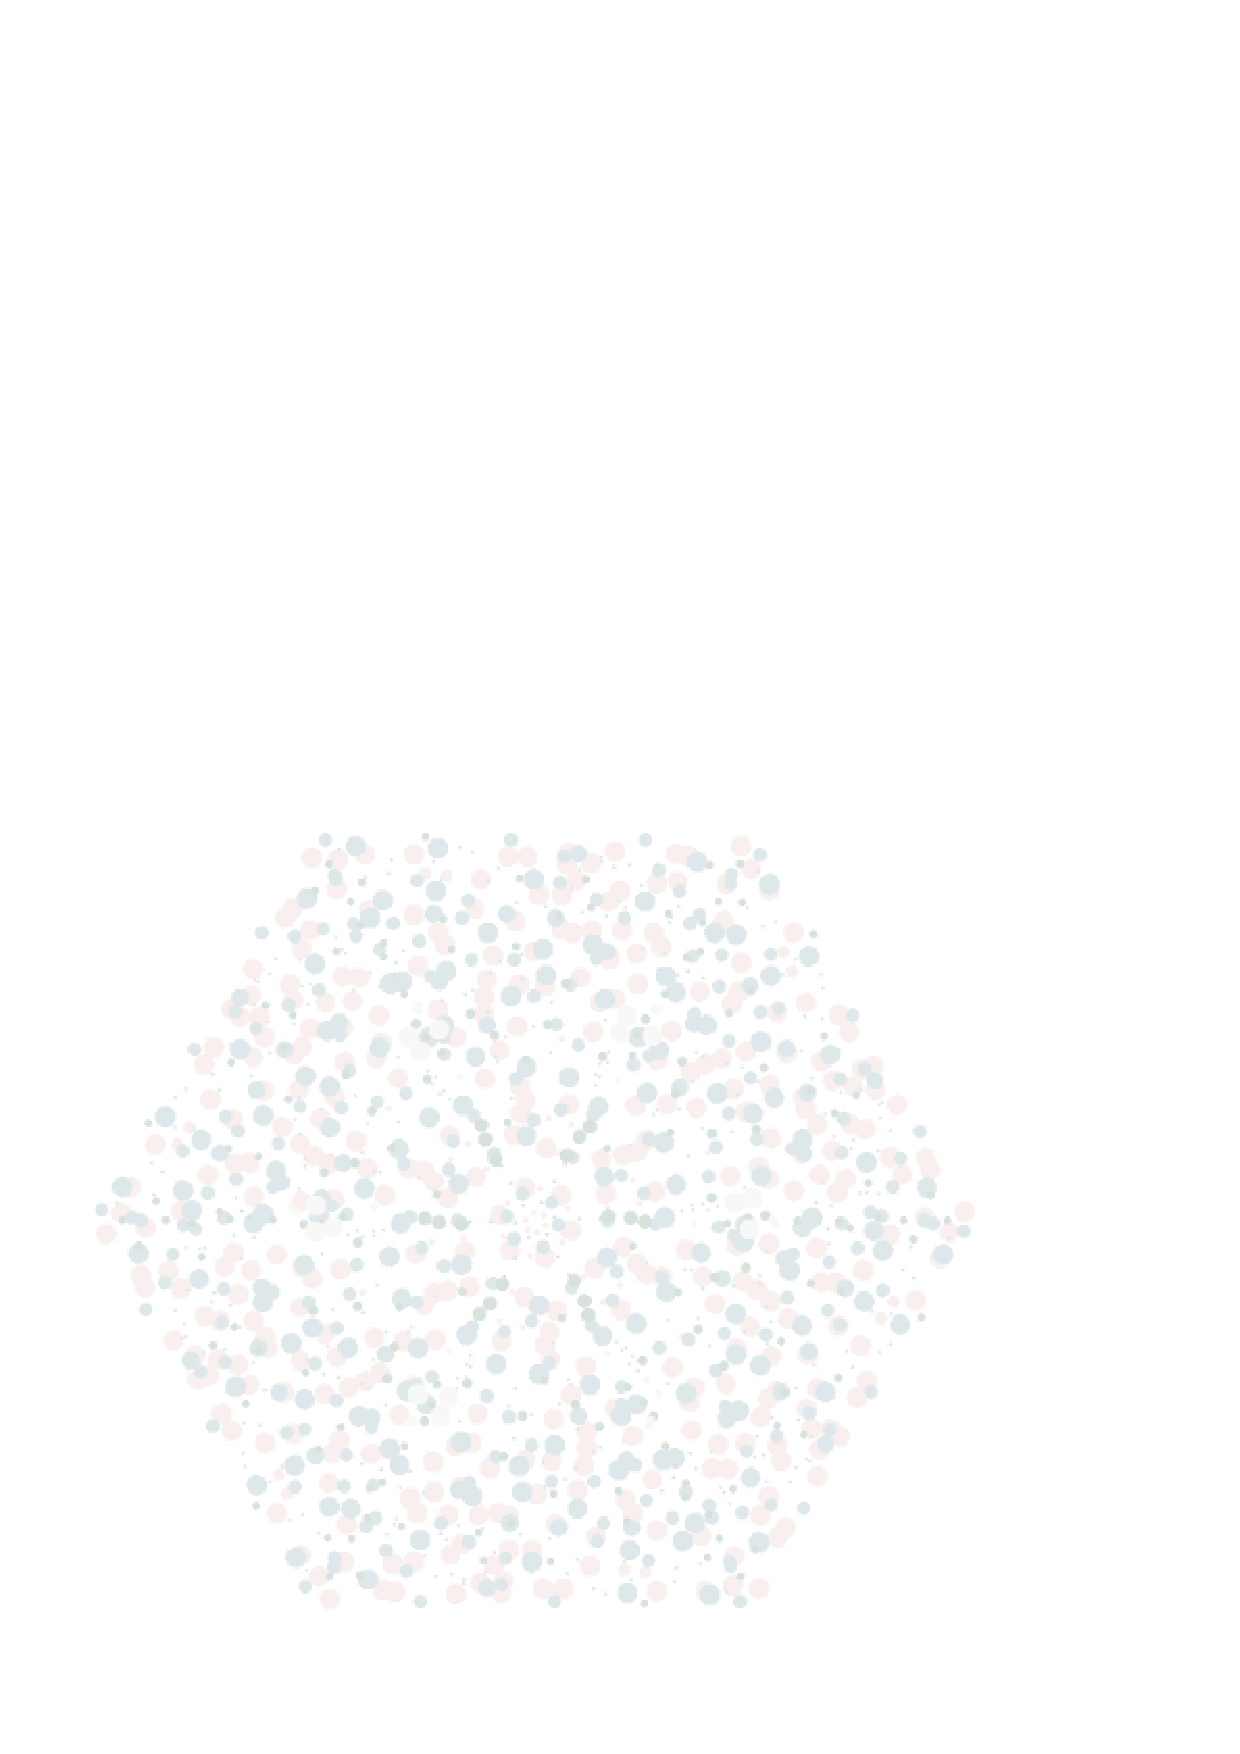
\includegraphics{flake}}\hfill}{}
\titlespacing{\section}{8cm}{1 cm}{-0.5 cm}
\titlespacing{\subsection}{8cm}{0.5 cm}{-0.5 cm}
\titleformat{\section}[awrap]{\large\bf\scshape}{\thesection}{1 em}{}{}
\titleformat{\subsection}[awrap]{\bf\scshape}{}{1 em}{}{}

%code listing:
\lstset{columns=fullflexible,
emph={apop_data,apop_model,apop_inventory,apop_estimate,apop_estimation_params,gsl_vector,gsl_matrix},emphstyle=\bf}
\def\setlistdefaults{\lstset{frame=single, showstringspaces=false, basicstyle=\small, language=C, breaklines=true}}
\setlistdefaults
%\def\cinline#1{\lstinline[language=C, showstringspaces=false, basicstyle=\small\bf,breaklines=true,breakatwhitespace=false,escapechar=\%]{#1}\setlistdefaults}
%\def\cinlinetwo#1{\lstinline[language=C, showstringspaces=false, basicstyle=\small\bf,breaklines=true,breakatwhitespace=false, escapechar=\%]{#1}}

\def\setc{\lstset{language=c}}
\def\setsql{\lstset{language=sql}}

%\def\cinline#1{{\tiny${}_\lfloor$}{#1}\nobreak\hskip 1pt\nobreak\raisebox{4pt}[0pt][0pt]{\tiny${}^\rceil$}}
\def\cinline#1{{\bf\tt #1}}
\def\binline#1{{\bf\tt #1}}
\def\sinline#1{{\bf\tt #1}}
\def\cinlinetwo#1{{\tt #1}}
\def\sinlinetwo#1{{\tt #1}}
\def\airq#1{{\sl #1}}

\long\def\codefig#1#2{
	\begin{figure}
	\hrule\vskip4pt
\lstset{frame=,showstringspaces=false, basicstyle=, language=C, breaklines=true}
\lstinputlisting{sources/#1.c}
	\hrule

	\caption{#2}\label{#1}
	\end{figure}
}

%indexing:
\usepackage{multicol, makeidx, url}
\usepackage[left=1.3in, right=1in,top=1in,bottom=1in]{geometry}
\makeindex
\def\ind#1{\index{#1}#1}
\def\ttind#1{\index{#1@\cinlinetwo{#1}}\cinline{#1}}
\def\cind#1{\index{#1@\cinlinetwo{#1}}\cinline{#1}}
\def\sqlind#1{\index{#1@\sinlinetwo{#1}}\sinline{#1}}
\def\ttindex#1{\index{#1@\cinlinetwo{#1}}}
\def\cindex#1{\index{#1@\cinlinetwo{#1}}}
\def\sindex#1{\index{#1@\sinlinetwo{#1}}}
%\def\ttind#1{\index{#1@{\tt #1}}{\tt #1}}
%\def\ttindex#1{\index{#1@{\tt #1}}}
\def\ff#1{#1 {\it ff}} %e.g. \index{pointers|ff}
\def\vocab#1{{\sl #1}\index{#1}}



%margin boxes:
\setlength\fboxsep{5pt} %margin size in margin boxes
\long\def\marginalia#1#2{
\begin{wrapfigure}{l}[1.3cm]{3in}
\fbox{\begin{minipage}{2.8in}
{\bf #1}\vskip .5cm\par
\small #2
\end{minipage}
}
\end{wrapfigure}
}

%title page:
\begin{document}
\frontmatter
\title{Statistical Computing}
\author{Ben Klemens\\klemens@hss.caltech.edu}
%\date{May 2005}
\date{February 2006}
\begin{center}
\fbox{\begin{minipage}{4in}
\maketitle
\end{minipage}}
\end{center}
\thispagestyle{empty}
\vfill
[A caveat: This book is very incomplete. The
first three chapters are finished, but it tapers off from there. It should
already have utility to many people, so it is here for your perusal.
This book plain old \copyright 2006, Ben Klemens.]
\comment{All the content in the preface is in chapter one.
\chapter*{Preface}
\input preface.tex
}
\setcounter{tocdepth}{1}
\tableofcontents
\mainmatter\chapter[Introduction]{Doing statistics in the modern day}
%\pagenumbering{arabic}\setcounter{page}{1}


In case it is not obvious to you, we can not do statistical analysis without
computers. The mathematical explanation of a statistical procedure is
really just pseudo-code, which we can make operational by translating
it into real computer code.

I wrote this book to help you make that translation. The first focus is purely
mathematical: we need to select techniques bearing in mind that they will eventually
be code. The second focus is about practical coding: your life
is short, and you want spend as little of it learning dumb languages as possible.

Doing math with a computer is unfettering. Instead of using
regression techniques designed before computers, we can use techniques
built around computing thousand-term likelihood functions, or taking
millions of random samples. These techniques originally appeared in the textbooks as
just theory, then eventually with a caveat that these techniques are possible but
computationally intensive. Now computations are cheap, and we can 
use these techniques as we would their simplified brethren.

In my own pain-filled experience, the best way to operationalize statistical concepts
is using C; the GNU Scientific Library,  which facilitates the linear
algebra and the Gaussian distribution work; and SQLite, a package which
facilitates handling large data sets. This book will cover the basics
of these components and the manner in which we can translate from the
mathematical language to the language these libraries speak.

The book is a complement to the Apophenia library, a set of functions 
based on the GSL and SQLite, intended to simplify the hard parts of
using these packages for statistical analysis. You could do all of the
analyses in this book without Apophenia, but you would find yourself
rewriting many of its functions. 
\comment{
Most stats packages include a manual that attempts to instruct the reader,
and an alphabetical-order reference providing detailed usage notes for
functions and structures.  You are reading Apophenia's manual now,
and the reference is online at \url{http://apophenia.info/doc}.}

This book falls in a mid-range between low-level numerical
computation and high-level use of prepackaged functions. For example,
{\sl Numerical Recipes in C} \citep{recipesinc} is a classic text
describing the algorithms for seeking optima and efficiently calculating
determinants. Being such a classic, there are many packages such as the
GSL that implement the algorithms from {\sl Numerical Recipes}, and this
book will build upon rather than replicate their effort. At the other
end, an abundance of texts will explain to readers how to do basic
statistics using the stats package of the month; this book lists the
one-line commands at this level, but it also breaks open the black boxes
and shows how those computations are done, so the reader can modify them
according to the vagaries of real-world data.

\paragraph{The intended audience}
I assume that you have had a statistics class already, but may need some refreshing
here and there, and so I will include digressions to remind you of your Greek. I also
assume that you are basically computer-literate, so I won't explain to you how to
turn on your computer, copy files, or work with a text editor.

There is an up-front investment to the methods here, and a long-term
payoff. If you expect that you will never do
anything more difficult than a linear regression on well-formed \ind{iid} data,
or if you are trying to slog through your department's stats requirement
so you can never look at another data set again, then by all means, put
this book down and get a copy of the easiest stats package you can get
away with. But if you expect to be doing statistical work for a larger
part of your career, such that problems of extensibility, portability,
and precision may be looming in your future, then this book is for you.

\section{The stats covered} 
As powerful as we like to think modern statistics is, it has a 
limited set of tricks at its disposal. For the purposes of this book,
I will divide them into three broad categories, which are broad enough
to cover the great majority of classical statistics (in fact, they overlap).

{\it Projections.} This includes the overused OLS linear regression (which is
a projection of your data onto a line), and the underused factor analysis
techniques. These are the techniques we humans use to reduce too many
dimensions down to something we can comprehend and even draw a picture of.

{\it Gaussian distribution tricks.} The Central Limit Theorem says that
a very wide range of statistics will have a Normal distribution. Square
the Normal, and we have a Chi-squared distribution. Take the ratio of two
Chi-squared distributions, and we have an F distribution.  The sum of
a random number of Normally distributed variables will have a Laplace
distribution.

{\it Likelihood function tricks.} Once we know the probability of an
event, probably thanks to a Gaussian distribution trick, we can then
write down the likelihood that a given set of parameters would bring
about the data we see, and then find the parameters that maximize this
likelihood. MLEs have the pleasing property of meeting the Cramer-Rao
lower bound, and the ratio of likelihood functions has the pleasant
property embodied in the Neyman-Pearson lemma, making them the basis of
hypotheses testing.

\subsection{The goals of statistics} Let's settle an
important fact about statistical analysis: it proves nothing, only
persuades. A large part of this is that we are looking for causal stories
about the world, but there is no statistical technique (and never will be)
that proves causality. Further, there is always a way to rewrite a model
or re-draw the data so that a rejected hypothesis is not, or vice versa.
But some results are more robust to tweaking 
than others, and some models are just plain more persuasive than others.

Within the overall goal of persuasion, we can subdivide the goals of
statistical analysis into two parts. The first is to just say something
interesting about a data set. This is often model-free; for example,
you may just want to show that two variables are highly correlated, or
that the data can mostly be described by three dimensions. This is often
sufficient to support an argument, and if that's the case, then you should
go no further in dazzling the reader with your statistical abilities.

The second part of statistical analysis is hypothesis testing, in which
we calculate a parameter of the data and then make a claim about that
parameter.  Having observed in the last paragraph that the correlation
coefficient of two variables is large, perhaps we would like to show
that that correlation coefficient is almost certainly different from
zero. More often, we have parameters in a model that we have written,
and would like to make claims about those parameters.

The techniques used for the two goals above are entirely different. For
example, there are any of a number of distributions listed in the
average stats textbook.  Poisson or Binomial distributions are used
only for describing data culled from the real world, while the Chi-squared
distribution or the F distribution are used only for testing hypotheses
about parameters we have written down ourselves (such as the correlation
coefficient, which has an F distribution). \cite{kmenta} points out that nothing
in nature has a Chi-squared distribution. 

Often, your work will shift
gears from describing the data (like fitting an OLS regression to the
data) to testing a hypothesis (like the claim that the coefficients
in your regression are significantly different from zero). Many stats
textbooks run these goals together at every opportunity;
hopefully I am doing better here, but it is up to you to know exactly
which goal you are working on with each line of code or math, and to be
certain that it is working toward your overall goal of saying something
interesting and persuasive.

\subsection{General theorems and their special cases}
Here is another way to subdivide the theorems that underly
statistics, this time into two classes. The first class, including the
results about MLEs, applies almost universally, but requires a huge
amount of computational power to arrive at a result. The second class
consists of special cases of these general results, such as the theorems
underlying OLS regressions (which are an application of the general
theorems behind the likelihood ratio test); these results impose more
assumptions, but are much easier to calculate, so that the results could
be used a century before computers were invented.

The second class is what we spend most of our time learning in school,
because a few decades ago, this was the only class of results which
civilians had the computing power to use. This is when the stats packages
that are so prevalent today came to the fore, automating the tedium of
applying these special case results. The technology had an immediate
influence on how people did research: they applied those darn special
cases to everything, and one would have a hard time finding an issue of an
academic journal today that doesn't have at least one OLS regression.
Everything in the world has become a linear process.

This book is about using OLS only when it is applicable. OLS was the only
viable tool for a hundred years or so, but we are done with using it everywhere.
The Central Limit Theorem tells us that yes, errors often are
Normally distributed; and it is often the case that yes, the dependent
variable is more or less a linear or log-linear function of several
variables. If such descriptions do no violence to the reality from
which the data was culled, then OLS is the method to use, and using
more general techniques will not be any more persuasive. But if these
assumptions are not true, then using OLS is at best unpersuasive, and at
worst disingenuous. Before computing power was where it is today, OLS was
as persuasive as we could get, and we all just had to accept that. But
now it is possible (and as this book hopes to show, even easy) to write
down exactly the right likelihood function, and to find exactly the best
parameters, instead of settling for the unpersuasive---and often
inapplicable---model which requires the least processor power.

\section{The programming covered}

Using C is a mix of low-level and high-level
work. You will be allocating memory, telling the computer exactly where
to shunt its electrons. But, thanks to the efforts of tens of thousands
of programmers before you, you will have the benefit of functions that
will find the minimum of a function or calculate characteristics of a
Normal distribution, without having to remember Newton's method or
the equation for the Gaussian distribution.

The first few chapters of this book will cover the basics of C itself,
in terms of its grammar and how to call those functions that
you will find to be so valuable. The remainder of the book will be at the higher
level, describing how to glue together the functions in the
GNU Scientific Library, SQLite, and Apophenia to get your research done.

\subsection{The computation engine} The GNU Scientific Library includes tools for
all of the procedures mentioned above: linear algebra operations, looking up the
value of F-, t-, $\chi^2$- distributions, calculating likelihood functions, and
maximizations. These will be the building blocks for analysis.

\subsection{Dealing with large data sets} More than anything, the problem
with stats packages is that large data sets can be hard to deal
with. Those languages designed around dealing with large data
sets tend to be even more draconian than C---for example, SAS's data
input command is {\tt card}, referring to the punch card it expects you
to put in the hopper.\footnote{SAS, by the way, gets its facility with large data sets
by providing a front-end to SQL queries. You can enter SQL directly into
SAS if you so choose.}

The best programs for large data sets are databases. They are designed
from the ground up to do nothing but let you efficiently retrieve what you
need from huge amounts of data.  Of course, being so purpose-specific,
there is no way to do statistics in a database (beyond trivialities like calculating
averages). Fortunately, we are working in C, so we can have the best of
all worlds. The method I advocate in this book (and the method that
Apophenia facilitates) is to read all of your
data into a database, and then query what you need to a matrix, as you
need it. This requires learning a new syntax, SQL, which is decidedly
neither Beautiful nor Perfect, and adds a level of complication on top
of what you are already dealing with. But the ease of manipulating data
sets offered by SQL is very much worth its short learning curve.

Apophenia  uses the SQLite library, which will
give you all the database functionality you need. Those of you who are
already database gurus, or who have data which is already handled
by another database engine, will easily be able to adapt the techniques
used here, but will need to brush up on the details of how to access
your site's database. Since you are using C instead of a stats package,
you are guaranteed that there is an interface out there that you can
download and incorporate into your programs.

\subsection{Pretty pictures} One thing C is not really good for is drawing
pretty pictures. This is not to be belittled, since those pictures
can be very persuasive. Consistent with the rest of this book, plotting
is done via Gnuplot, a program which is freely available for
the system you are using right now. Gnuplot is highly automatable, so once
you have a plot you like, you can have your C programs autogenerate
it or manipulate it in cute ways, or can send your program to your
colleague in Madras and he will have no problem reproducing and modifying
your graphs.

\input why_c.tex


\section{Outline} 
Part I covers general scientific computing, and will be valuable to
anyone who needs to program a computer to handle and do math with large volumes of data.
Since I am assuming that you are computer-literate but
not a C programmer, Chapter \ref{c_crash} will give you a crash course
in C. It will not only get you familiar with the rules of the language,
but how to best think about problems in C. 
Chapter \ref{sql} will give you a quick overview of the second language,
Standard Query Language (SQL), which is a language that facilitates
producing tables of just the right form from a dataset. C and SQL are
excellent complements for data analysis: things which are very difficult
in one are often trivial in the other.
Chapter \ref{linear_algebra}
will then introduce you to the package of C functions most useful for
doing stats: the GNU Scientific Library (GSL). Notably, it will cover
how to do linear algebra using the GSL. Chapter \ref{apop} covers
Apophenia, a library of functions that bind together the GSL and SQLite
to facilitate data handling and statistics.


Given those tools, coding statistics will be easy. Part II includes a chapter
devoted to each of the three categories of statistics above: Chapter \ref{projections}
handles the process of describing your data, using simple calculations
or projection techniques; Chapter
\ref{gauss} covers methods of comparing your data to various Gaussian
distributions, such as the t test, F test, and chi-squared test; Chapter
\ref{mle} will show you how to write down your likelihood functions and
find their maxima, as in Probit or Normit estimations, and how to test
hypotheses using a likelihood ratio test. Chapter \ref{boot} will cover
bootstrapping and jackknifing, which are dirty tricks which will one
day save your life.  Finally, Chapter \ref{gnuplot} will cover creative
uses of Gnuplot to display data.

When you are done with all this---and this is no exaggeration---you will
have the tools to implement any technique in classical statistics in
existence today, on any data set, no matter how large or exceptional.
\part{Computing}
\input c_crash.tex
\input sql.tex
\input linear_algebra.tex
\input apop.tex
\part{Statistics}
\input projection.tex
\input gauss.tex
\input mle.tex
\input boot.tex
%\input mcmc.tex
\input gnuplot.tex
\nocite{*}
\backmatter
\bibliographystyle{plainnat}
\bibliography{guide}
\printindex
\end{document}
